%!TEX program = lualatex

% Unofficial MSU Poster template.
% A fork of https://www.overleaf.com/latex/templates/an-unofficial-poster-template-for-new-york-university/krgqtqmzdqhg
% ...which is a fork of https://github.com/anishathalye/gemini
% also refer to https://github.com/k4rtik/uchicago-poster



\documentclass[final]{beamer}

% ====================
% Packages
% ====================

\usepackage[T1]{fontenc}
 \usepackage[utf8]{luainputenc}
\usepackage{lmodern}
\usepackage[size=custom, width=120,height=72, scale=1]{beamerposter}
\usetheme{gemini}
\usecolortheme{msu} % remove to avoid the sheeshee effect
\usepackage{graphicx} 
\usepackage{booktabs}
\usepackage{tikz}
\usepackage{pgfplots}
\pgfplotsset{compat=1.14}
\usepackage{anyfontsize}

% ====================
% Lengths
% ====================

% If you have N columns, choose \sepwidth and \colwidth such that
% (N+1)*\sepwidth + N*\colwidth = \paperwidth
\newlength{\sepwidth}
\newlength{\colwidth}
\setlength{\sepwidth}{0.025\paperwidth}
\setlength{\colwidth}{0.3\paperwidth}

\newcommand{\separatorcolumn}{\begin{column}{\sepwidth}\end{column}}

% ====================
% Title
% ====================

\title{Homotopy Continuation in Economics}
\author{Kevin Phan (Under Dr. Max Hill)}

% I would like to thank Dr. Max Hill for his support through this project. 

\institute[shortinst]{Department of Mathematics, University of Hawaiʻi at M\=anoa}


% ====================
% Footer (optional)
% ====================

\footercontent{
  \href{https://github.com/kevinphan981/homotopycontinuation-econ}{github.com/kevinphan981/homotopycontinuation-econ} \hfill
  \href{mailto:youremail@msu.edu}{phank9@hawaii.edu}}
% (can be left out to remove footer)

% ====================
% Logo (optional)
% ====================
\usepackage{svg}
% \usepackage[absolute,overlay]{textpos}
% use this to include logos on the left and/or right side of the header:
% Left: institution
 \logoright{
\includegraphics[height=9cm]{logos/uhm-logo-huge.png}}
% Right: funding agencies and other affilations 
%\logoright{\includegraphics[height=7cm]{logos/NSF.eps}}
% ====================
% Body
% ====================

\begin{document}



\begin{frame}[t]
\begin{columns}[t]
\separatorcolumn

\begin{column}{\colwidth}

  \begin{block}{What is Homotopy Continuation?}

    \begin{figure}
      \centering
        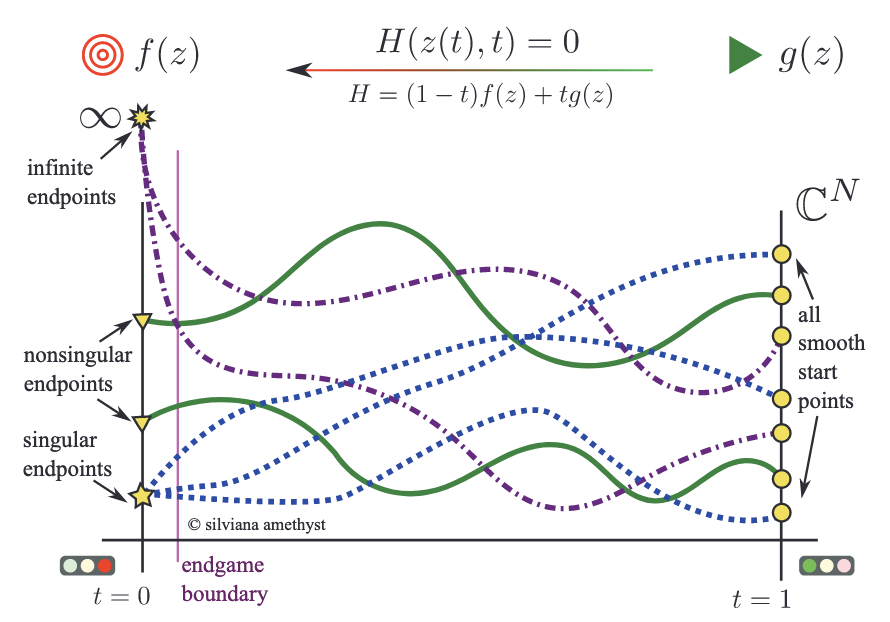
\includegraphics[width=0.65\textwidth]{figures/duff-diagram-basic.png}
        \caption{Illustrative Example from Duff \& Regan}
    \end{figure}

    Homotopy Continuation is a numerical method that leverages concepts from algebraic geometry to 
    solve nonlinear systems of polynomial equations. There are many examples ranging from Physics, Robotics, Ecology, 
    and in this poster, Economics. We will use the programming language Julia with the library HomotopyContinuation.jl.

  \end{block}


  \begin{alertblock}{Background}

      A homotopy is a continuous function $H$ between two continuous functions $f, g$ from the topological spaces $X$ and $Y$ such that  $$H: X \times [0,1] \to Y$$
      such that $H(x, 0) = f(x)$ and $H(x,1) = g(x)$ for all $x \in X$.

    \begin{itemize}
      \item A system of equations $g(\boldsymbol{z}) = 0$ where the solutions are known is called the \textbf{start system}. 

      \item The system of equations that we want to eventually reach (with continuous deformation) is the 
      \textbf{target system}, another system of equations $f(\boldsymbol{z}) = 0$, whose solutions we want to know.

    \end{itemize}

    There are several types of homotopies and ways to compute solutions. For now, we will focus on the \textbf{Total Degree Homotopy} that uses an intuitive start system.
  \end{alertblock}

  \begin{exampleblock}{Example of Total Degree Homotopy}
    \begin{equation*}
        f(x,y) = 
        \begin{pmatrix}
            x^2 + y^2 - 3 \\
            2x^2 + 0.5x*y + 3y^2 - 2
        \end{pmatrix}
    \end{equation*}

    And the corresponding total degree start system. 

    \begin{equation*}
        g(x,y) = 
        \begin{pmatrix}
            x^2 - 1 \\
            y^2 - 1
        \end{pmatrix}
    \end{equation*}

    We have (1,1), (-1,1), (1,-1), (-1,-1) as starting solutions.

  \end{exampleblock}  

  
\end{column}

\separatorcolumn

\begin{column}{\colwidth}

  \begin{block}{Example Results}

    Fortunately, this example is quite simple. 
    There are four non-singular paths that are real. However, the solutions are actually complex.


    \begin{table}[h]
    \centering
    \renewcommand{\arraystretch}{1.3}
    \begin{tabular}{ccc}
        \toprule
        \textbf{Solution} & \textbf{$x$ Coordinate} & \textbf{$y$ Coordinate} \\ 
        \midrule
        1 & $2.47 - 0.42i$ & $-0.58 - 1.80i$ \\
        2 & $-2.47 - 0.42i$ & $0.58 - 1.80i$ \\
        3 & $2.47 + 0.42i$ & $-0.58 + 1.80i$ \\
        4 & $-2.47 + 0.42i$ & $0.58 + 1.80i$ \\
        \bottomrule
      \end{tabular}
      \caption{Complex Solutions for the Initial System $f$}
    \end{table} 
    
    \begin{figure}
      \centering
        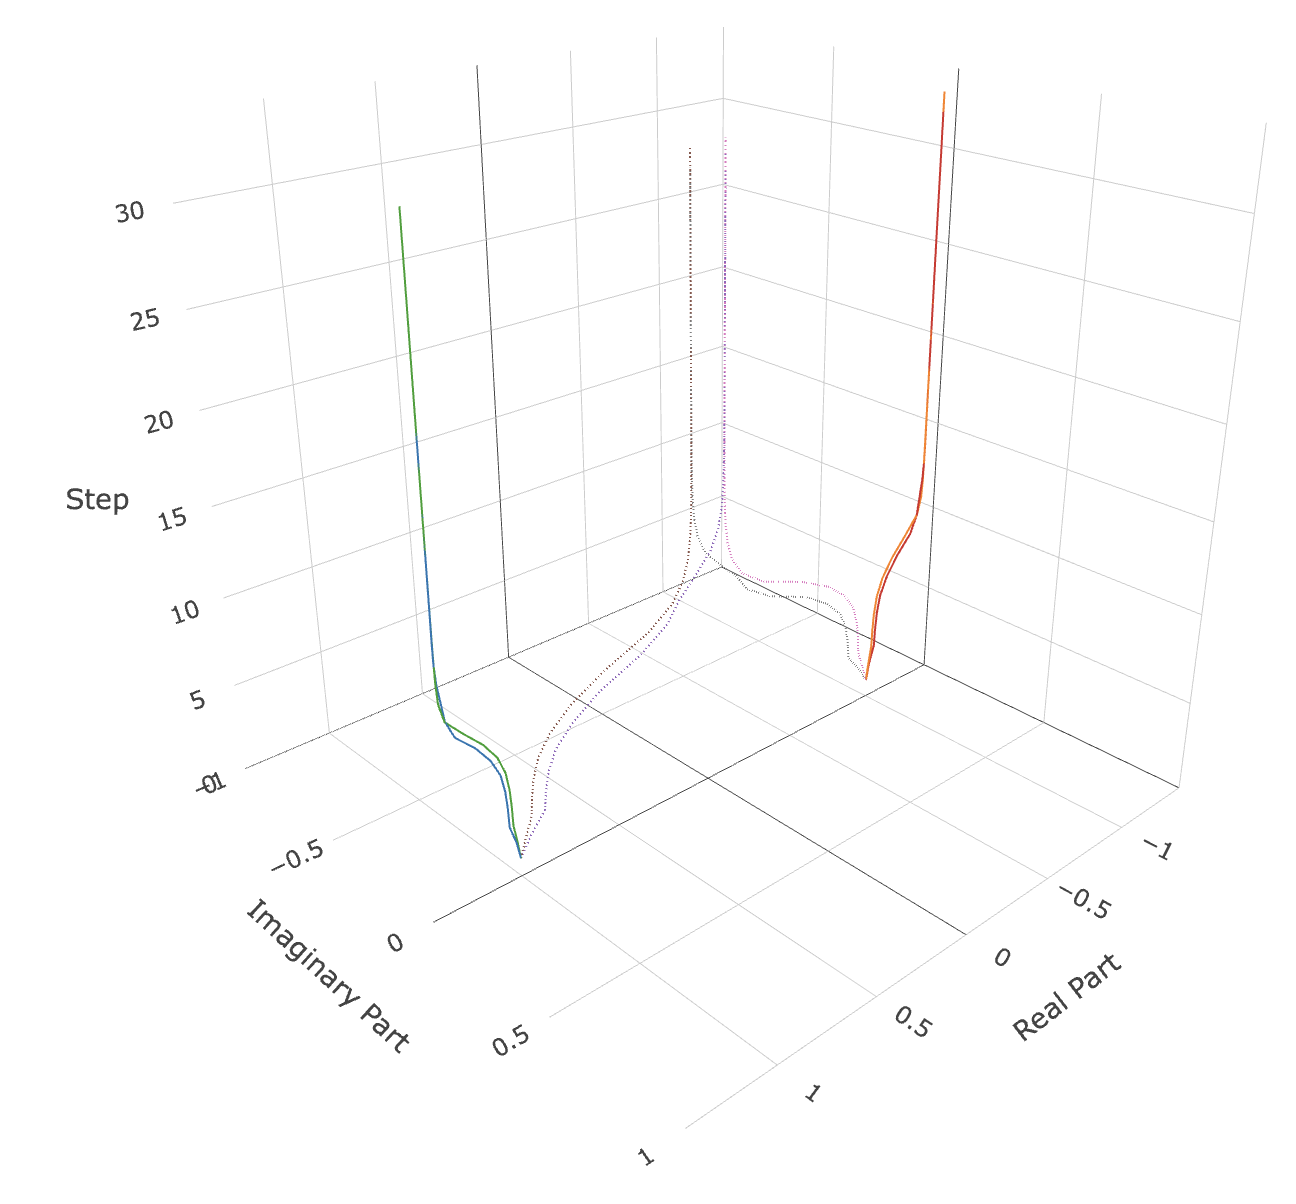
\includegraphics[width=0.65\textwidth]{figures/test2-true.png}
        \caption{Simple Example Visualized (Bold: x, Dotted: y)}
    \end{figure}

  \end{block}

  \begin{alertblock}{The Bertrand Model}

    Given two firms (a duopoly) that are subject to different consumers/products (and consequently different demand curves), 
    they attempt to find a pure-strategy Nash equilibrium where they maximize profit. 

    We will consider an example that was created into a systems of polynomial equations below, 

    \begin{align*}
        f_1 &= -2700 + 2700p_x + 8100Z^2p_x^2 - 5400Z^2p_x^3 + 51Z^3p_x^6 - 2Z^3p_x^7 \\
        f_2 &= -2700 + 2700*p_y + 8100Z^2p_y^2 - 5400Z^2*p_y^3 + 51Z^3p_y^6 - 2Z^3p_y^7 \\
        Z &= Z^2 p_x^2 p_y^2 - (p_x^2 + p_y^2)
    \end{align*}

    Additionally, we also use some first and second order conditions to narrow down our solutions. 
    For example, negative or infinite solutions are not valid for Economics.
  \end{alertblock}

\end{column}

\separatorcolumn

\begin{column}{\colwidth}


  \begin{block}{Results of Bertrand Model with Homotopy Continuation}
    In the graph below, there are 600 solutions that are generated, but many of them veer of into infinity and are not relevant.

    \begin{figure}
      \centering
        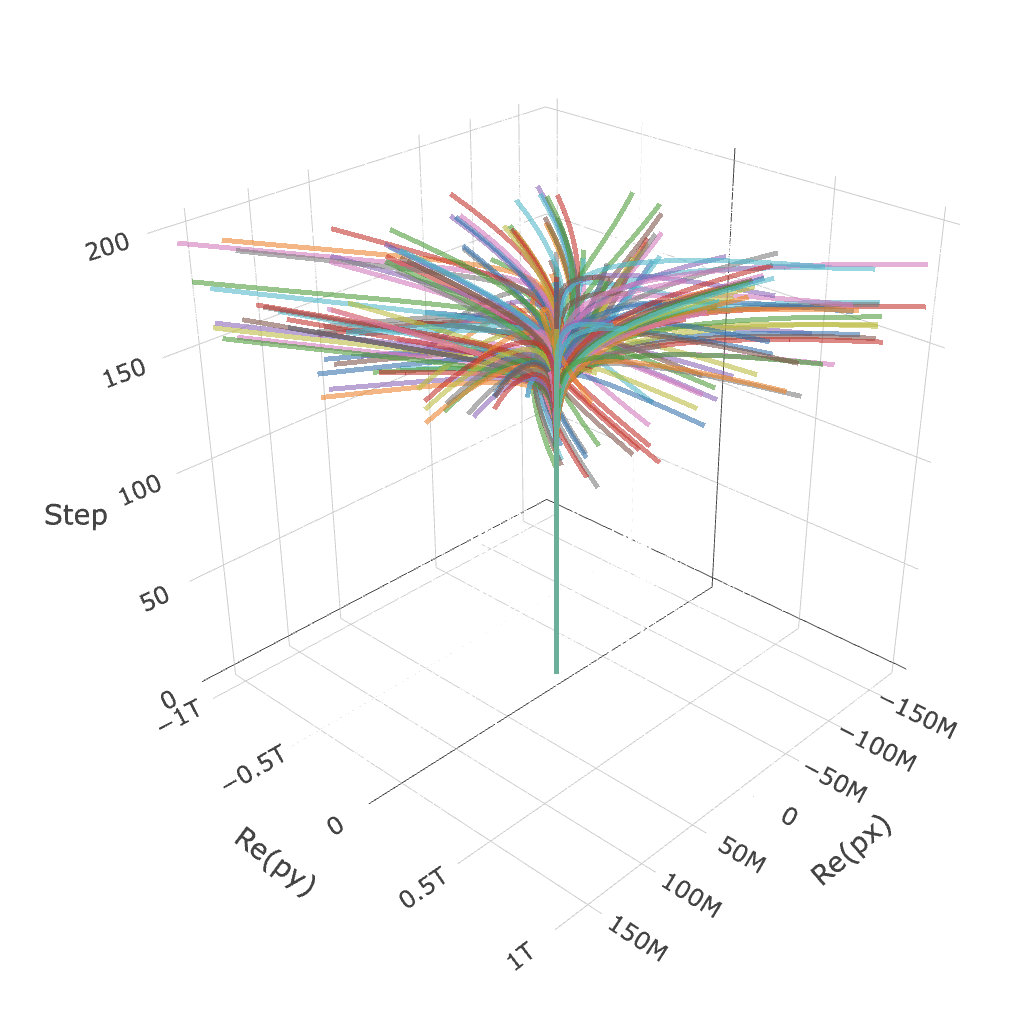
\includegraphics[width=0.65\textwidth]{figures/bertrand-prices.png}
      \caption{Results of Bertrand Model with Homotopy Continuation}
    \end{figure}

    We use Julia and filter out solutions based on being real, positive, and satisfying the 
    second-order condition of the firms. In general we get 62 solutions, 18 real. But there are only 4 relevant solutions.
  \begin{table}[h]
      \centering
      \renewcommand{\arraystretch}{1.5} % Adds vertical breathing room
      \begin{tabular}{cc}
          \toprule
          \multicolumn{2}{c}{\textbf{Equilibrium Prices}} \\ 
          \midrule
          $(p^1_x, p^1_y) = (1.757, 1.757)$ & $(p^2_x, p^2_y) = (22.987, 22.987)$ \\
          $(p^3_x, p^3_y) = (2.168, 25.157)$ & $(p^4_x, p^4_y) = (25.157, 2.168)$ \\
          \bottomrule
      \end{tabular}
      \caption{Relevant Strategies for the Bertrand Model}
  \end{table}

  \end{block}

  \begin{block}{References}
    \nocite{*}
    % \footnotesize{\bibliographystyle{plain}\bibliography{poster}}

    \footnotesize
    \bibliographystyle{abbrv} % or alpha, plain, etc.
    \bibliography{poster}      % This must match your filename "poster.bib"
    
  \end{block}

\end{column}

\separatorcolumn
\end{columns}
\end{frame}

\end{document}
